\clearpage
\section{Tool availability and implementation}
\label{sec.tool}
\smashpp is implemented in \cpp language and is available at~\cite{web-smashpp}. This tool is able to find and visualize rearrangements in sequences, \fasta and \fastq files; although, it is highly recommended to use sequences as input. In the following sections, we describe installing and running the \smashpp tool.

\subsection{Install}
To install \smashpp on various operating systems, follow the instructions below. Note that the precompiled executables are available for 64 bit operating systems in the ``bin/'' directory.

% \paragraph{Conda}
% % todo

\paragraph{Linux}
\begin{itemize}
  \item Install ``git'' and ``cmake'':
\begin{code}[style=bash]
sudo apt update
sudo apt install git cmake
\end{code}
\item Clone \smashpp and install it:
\begin{code}[style=bash]
git clone https://github.com/smortezah/smashpp.git
cd smashpp
./install.sh
\end{code}
\end{itemize}

\paragraph{macOS}
\begin{itemize}
    \item Install ``Homebrew'', ``git'' and ``cmake'':
\begin{code}[style=bash]
/usr/bin/ruby -e "$(curl -fsSL https://raw.githubusercontent.com/Homebrew/install/master/install)"
brew install git cmake
\end{code}
\item Clone \smashpp and install it:
\begin{code}[style=bash]
git clone https://github.com/smortezah/smashpp.git
cd smashpp
./install.sh
\end{code}
\end{itemize}

\paragraph{Windows}
\begin{itemize}
  \item Download and install ``CMake'', e.g., from https://github.com/Kitware/CMake/releases/\linebreak download/v3.14.4/cmake-3.14.4-win64-x64.msi. Make sure to add it to the system PATH. For example, if CMake is installed in ``C:\textbackslash Program Files'', add ``C:\textbackslash Program Files\textbackslash CMake\textbackslash bin'' to the system PATH.
  \item Download and install ``mingw-w64'', e.g., from https://sourceforge.net/projects/mingw-w64/\linebreak files/latest/download. Make sure to add it to the system PATH. For example, if it is installed in ``C:\textbackslash mingw-w64'', add ``C:\textbackslash mingw-w64\textbackslash mingw64\textbackslash bin'' to the system PATH.
  \item Download and install ``git'', from https://git-scm.com/download/win.
  \item Clone \smashpp and install it:
\begin{code}[style=bash]
git clone https://github.com/smortezah/smashpp.git
cd smashpp
.\install.bat
\end{code}
\end{itemize}

\subsection{Run}
A reference file and a target file are clearly mandatory to run \smashpp (without visualization). Running
\begin{code}[style=bash]
./smashpp
\end{code}
provides the following guide:
%\vskip2mm
% \begin{code}[style=bash]
%   SYNOPSIS
%   ./smashpp  OPTIONS...  -r REF-FILE  -t TAR-FILE

%   SAMPLE

%   DESCRIPTION
%   Mandatory arguments
%   -r,  --ref FILE            reference file (Seq/Fasta/Fastq)
%   -t,  --tar FILE            target file    (Seq/Fasta/Fastq)

%   Options
%   -v,  --verbose             more information
%   -l,  --level INT           level of compression: [0, 5]
%   -m,  --min   INT           min segment size: [1, 4294967295]
%   -nr, --no-redun            do NOT compute self complexity
%   -e,  --ent-n FLOAT         Entropy of 'N's: [0.0, 100.0]
%   -n,  --nthr  INT           number of threads: [1, 8]
%   -fs, --filter-scale S|M|L  scale of the filter:
%   {S|small, M|medium, L|large}
%   -w,  --filt_size INT           window size: [1, 4294967295]
%   -wt, --filt_type INT/STRING    type of windowing function:
%   {0|rectangular, 1|hamming, 2|hann,
%   3|blackman, 4|triangular, 5|welch,
%   6|sine, 7|nuttall}
%   -d,  --step   INT          sampling steps
%   -th, --thresh FLOAT        threshold: [0.0, 20.0]
%   -sb, --save-seq            save sequence (input: Fasta/Fastq)
%   -sp, --save-profile        save profile (*.prf)
%   -sf, --save-filter         save filtered file (*.fil)
%   -ss, --save-segment        save segmented files (*-s_i)
%   -sa, --save-all            save profile, filetered and
%   segmented files
%   -h,  --help                usage guide
%   -rm, --ref-model  k,[w,d,]ir,a,g/t,ir,a,g:...
%   -tm, --tar-model  k,[w,d,]ir,a,g/t,ir,a,g:...
%   parameters of models
%   (INT) k:  context size
%   (INT) w:  width of sketch in log2 form,
%   e.g., set 10 for w=2^10=1024
%   (INT) d:  depth of sketch
%   (INT) ir: inverted repeat: {0, 1, 2}
%   0: regular (not inverted)
%   1: inverted, solely
%   2: both regular and inverted
%   (FLOAT) a:  estimator
%   (FLOAT) g:  forgetting factor: [0.0, 1.0)
%   (INT) t:  threshold (no. substitutions)
% \end{code}

\begin{code}[style=bash]
SYNOPSIS
  ./smashpp [OPTIONS]  -r <REF-FILE>  -t <TAR-FILE>

OPTIONS
  Required:
  -r  <FILE>         = reference file (Seq/FASTA/FASTQ)
  -t  <FILE>         = target file    (Seq/FASTA/FASTQ)

  Optional:
  -l  <INT>          = level of compression: [0, 5]. Default -> 0
  -m  <INT>          = min segment size: [1, 4294967295]     -> 50
  -e  <FLOAT>        = entropy of 'N's: [0.0, 100.0]         -> 2.0
  -n  <INT>          = number of threads: [1, 8]             -> 4
  -f  <INT>          = filter size: [1, 4294967295]          -> 256
  -ft <INT/STRING>   = filter type (windowing function):     -> hann
                       {0|rectangular, 1|hamming, 2|hann,
                       3|blackman, 4|triangular, 5|welch,
                       6|sine, 7|nuttall}
  -fs [S][M][L]      = filter scale:                         -> L
                       {S|small, M|medium, L|large}
  -d  <INT>          = sampling steps                        -> 1
  -th <FLOAT>        = threshold: [0.0, 20.0]                -> 1.5
  -rb <INT>          = ref beginning guard: [-32768, 32767]  -> 0
  -re <INT>          = ref ending guard: [-32768, 32767]     -> 0
  -tb <INT>          = tar beginning guard: [-32768, 32767]  -> 0
  -te <INT>          = tar ending guard: [-32768, 32767]     -> 0
  -dp                = deep compression                      -> no
  -nr                = do NOT compute self complexity        -> no
  -sb                = save sequence (input: FASTA/FASTQ)    -> no
  -sp                = save profile (*.prf)                  -> no
  -sf                = save filtered file (*.fil)            -> no
  -ss                = save segmented files (*.s[i])         -> no
  -sa                = save profile, filetered and           -> no
                       segmented files
  -rm k,[w,d,]ir,a,g/t,ir,a,g:...
  -tm k,[w,d,]ir,a,g/t,ir,a,g:...
                     = parameters of models
                <INT>  k:  context size
                <INT>  w:  width of sketch in log2 form,
                           e.g., set 10 for w=2^10=1024
                <INT>  d:  depth of sketch
                <INT>  ir: inverted repeat: {0, 1, 2}
                           0: regular (not inverted)
                           1: inverted, solely
                           2: both regular and inverted
              <FLOAT>  a:  estimator
              <FLOAT>  g:  forgetting factor: [0.0, 1.0)
                <INT>  t:  threshold (no. substitutions)
  -ll                = list of compression levels
  -h                 = usage guide
  -v                 = more information
  --version          = show version
\end{code}

The arguments ``-r'' and ``-t'' are used to specify the reference and the target, respectively, which are highly recommended to have short names. 
Level of compression, that is an integer between 0 and 5, can be determined with ``-l''. 
By setting ``-m'' to an integer value, only those regions in the reference file that are bigger than that value would be able to be considered for compression.

In implementation of the reference-based compression, we have replaced `N' bases in the references and the targets with `A's and `T's, respectively. On reference-free compression, they are replaced with `A's, in both references and targets. If a user tends to replace `N' bases in a sequence with a normal distribution of `A', `C', `G' and `T's, he/she can employ GOOSE toolkit~\cite{web-goose}. Note that we have set by default the entropy of `N's to 2.0, however, it can be changed to a value of interest using ``-e'' option.

Creating multiple finite-context models and substitutional-tolerant Markov models can be done in a multi-threaded fashion by setting ``-n'' to an integer. 

In the process of finding similar regions in the reference and the target sequences, the information content that would be obtained by compression needs to be filtered. Size of the window and type of the windowing function can be set by ``-f'' and ``-ft'' options, respectively.
Besides Hann window that is used by default to smooth the information content (profile), we have implemented several other windowing functions, including Blackman~\cite{blackman1959particular}, Hamming~\cite{tukey1949measuring}, Nuttall~\cite{nuttall1981some}, rectangular~\cite{oppenheim1999discrete}, sine~\cite{harris1978use}, triangular~\cite{bartlett1950periodogram} and Welch~\cite{welch1967use} windows. These functions are given by
\begin{align}
  w[n] & = 1,
  \tag*{(rectangular)}                                                                                                                                        \\
  w[n] & = 1-\left|\tfrac {n-N/2}{L/2}\right|, \quad L=N,
  \tag*{(triangular/Bartlett)}                                                                                                                                \\
  w[n] & = 1-\left(\tfrac {n-N/2}{N/2}\right)^{2},
  \tag*{(Welch)}                                                                                                                                              \\
  w[n] & = \sin \left(\tfrac {\pi n}{N}\right),
  \tag*{(sine)}                                                                                                                                               \\
  w[n] & = 0.54348-0.45652\;\cos \left(\tfrac {2\pi n}{N}\right),
  \tag*{(Hamming)}                                                                                                                                            \\
  w[n] & = 0.42659-0.49656\;\cos \left(\tfrac {2\pi n}{N}\right)+0.07685\;\cos \left(\tfrac {4\pi n}{N}\right),
  \tag*{(Blackman)}                                                                                                                                           \\
  w[n] & = 0.35577-0.48740\;\cos \left(\tfrac {2\pi n}{N}\right)+0.14423\;\cos \left(\tfrac {4\pi n}{N}\right)-0.01260\;\cos \left(\tfrac {6\pi n}{N}\right),
  \tag*{(Nuttall)}                                                                                                                                            \\
\end{align}
and are plotted in Fig.~\ref{fig.filters}.
Scale of the filter can be set as S (small), M (medium) or L (large), using ``-fs''.
Also, instead of considering the whole information content, the user is able to make samples of it by steps of which size can be determined by ``-d''.
\begin{figure}[!h]
  \centering
  \includegraphics[width=\linewidth]{filters.pdf}
  \caption{Window functions.}
  \label{fig.filters}
\end{figure}

For the purpose of segmenting the filtered information content, the average entropy of reference-based compression is used by default as the threshold, but the threshold can be altered by ``-th'' option.

\smashpp is capable of finding even small similar regions in two sequences. However, there are some corner cases that the size of similar regions in reference and target are not balanced. \smashpp handles these cases using ``-rb'', ``-re'', ``-tb'' and ``-te'' options, that can resize the beginning and ending guards of reference and target regions, respectively.
For example, if ``-tb 10'' is used, the first 10 bases in each target region will be ignored, which results in smaller regions.
Note that when \smashpp wants to create the model of each target region to use it for compression of the reference
% Note that using this option will affect the model that would be created 

-dp

Triggering ``-nr'' makes the tool not to perform the reference-free compression, self-complexity computation.

\smashpp accepts \fasta and \fastq files as input, in addition to sequences. In these cases, the input files are first converted to sequences and then processed further. It is possible to save these sequences by ``-sb'' option.
When the information profile is obtained, \smashpp smoothens then removes it by default. However, it can be preserved by ``-sp'' option.
The same thing happens to the smoothed file, i.e., it is segmented then removed. But, the user can use ``-sf'' to save the filtered file. 
Also, the segmented files can be saved using ``-ss''. 
The user can save all the information profile (content), filtered and segmented files, by triggering ``-sa'' option.

For the purpose of compression, it is recommended to use ``-l'' option, since it configures the models automatically. However, using ``-rm'' and ``-tm'', the user would be able to manually configure the reference model, for reference-based compression, and the target model, for reference-free compression, respectively. Parameters of the models are described in detail in section~\ref{sec.methods}.
Note that using ``-ll'' option, the list of parameters that would be chosen for each model automatically, will be shown.

Running \smashpp (without visualization), positions of the similar regions in the reference and the target, and also complexity of the regions is saved in a ``*.pos'' file. This file can be visualized by
\begin{code}[style=bash]
  ./smashpp -viz
\end{code}
which gives
% \begin{code}[style=bash]
%   SYNOPSIS
%   ./smashpp -viz  OPTIONS...  -o SVG-FILE  POS-FILE

%   SAMPLE

%   DESCRIPTION
%   Mandatory arguments:
%   POS-FILE                 positions file, generated by
%   Smash++ tool (*.pos)

%   Options:
%   -v,  --verbose           more information
%   -o,  --out SVG-FILE      output image name (*.svg)
%   -rn, --ref-name STRING   reference name shown on output. If name
%   has space, use "s, e.g. "Seq label".
%   Default: name in header of position file.
%   -tn, --tar-name STRING   target name shown on output
%   -vv, --vertical          vertical view
%   -nn, --no-nrc            do NOT show normalized
%   relative compression (NRC)
%   -nr, --no-redun          do NOT show self complexity
%   -ni, --no-inv            do NOT show inverse maps
%   -ng, --no-reg            do NOT show regular maps
%   -l,  --link     INT      type of the link between maps: [1, 6]
%   -c,  --color    INT      color mode: [0, 2]
%   -p,  --opacity  FLOAT    opacity: [0.0, 1.0]
%   -w,  --width    INT      width of the sequence: [15, 100]
%   -s,  --space    INT      space between sequences: [15, 200]
%   -f,  --mult     INT      multiplication factor for
%   color ID: [1, 255]
%   -b,  --begin    INT      beginning of color ID: [0, 255]
%   -rt, --ref-tick INT      reference tick: [1, 4294967295]
%   -tt, --tar-tick INT      target tick: [1, 4294967295]
%   -th, --tick-human 0|1    tick human readable: 0=false, 1=true
%   -m,  --min      INT      minimum block size: [1, 4294967295]
%   -h,  --help              usage guide
% \end{code}
\begin{code}[style=bash]
SYNOPSIS
  ./smashpp -viz [OPTIONS]  -o <SVG-FILE>  <POS-FILE>

OPTIONS
  Required:
  <POS-FILE>         = position file, generated by
                       Smash++ tool (*.pos)

  Optional:
  -o  <SVG-FILE>     = output image name (*.svg)             -> map.svg
  -rn <STRING>       = reference name shown on output. If it
                       has space, use double quotes, e.g.
                       "Seq label". Default: name in header
                       of position file
  -tn <STRING>       = target name shown on output
  -l  <INT>          = type of the link between maps: [1, 6] -> 1
  -c  <INT>          = color mode: [0, 1]                    -> 0
  -p  <FLOAT>        = opacity: [0.0, 1.0]                   -> 0.9
  -w  <INT>          = width of the sequence: [15, 100]      -> 16
  -s  <INT>          = space between sequences: [15, 200]    -> 62
  -f  <INT>          = multiplication factor for             -> 43
                       color ID: [1, 255]
  -b  <INT>          = beginning of color ID: [0, 255]       -> 0
  -rt <INT>          = reference tick: [1, 4294967295]
  -tt <INT>          = target tick: [1, 4294967295]
  -th [0][1]         = tick human readable: 0=false, 1=true  -> 1
  -m  <INT>          = minimum block size: [1, 4294967295]   -> 1
  -vv                = vertical view                         -> no
  -nn                = do NOT show normalized relative       -> no
                       compression (NRC)
  -nr                = do NOT show self complexity           -> no
  -ni                = do NOT show inverse maps              -> no
  -ng                = do NOT show regular maps              -> no
  -h                 = usage guide
  -v                 = more information
  --version          = show version
\end{code}

The output of \smashpp visualizer is an ``SVG'' file, which its name is determined by ``-o'' option. By default, it is named ``map.svg''. Names of the reference and the target, which are going to be printed on the output image, can be altered by ``-rn'' and ``-tn'', respectively. They are by default the names written in the positions file. To have a vertical view of the image, instead of the default horizontal view, one can use ``-vv'' trigger.

\smashpp performs reference-based and reference-free compressions to calculate the normalized relative compression (NRC) and redundancy (self complexity), respectively. If the user is not interested in showing them, he/she can turn them off by ``-nn'' and ``-nr'' triggers. In addition, \smashpp considers both regular and reverse complement maps by default in its calculations. Triggering ``-ni'' and ``-ng'' will stop showing inverted and regular maps, respectively.

Options ``-l'', ``-c'', ``-p'', ``-w'', ``-s'', ``-f'' and ``-b'' can be used to change the appearance of the image. Assigning integers to ``-rt'' and ``-tt'' options will change the tick sizes of the reference and the target, respectively. \smashpp prints the sizes on axes in human readable format, e.g., 1K, 2M, etc. However, it can be triggered by ``-th'' option. Note that, here, 1K is equivalent to 1000 and not 1024. Finally, by setting ``-m'' to an integer value, only the regions that are bigger than that value will be illustrated.

\subsection{Example}
This section guides, step-by-step, employing \smashpp to find and visualize rearrangements in a sample genomic data.

\subsubsection*{Install \smashpp and provide the required files}
First, we install \smashpp:
\begin{code}[style=bash]
  git clone https://github.com/smortezah/smashpp.git
  cd smashpp
  ./install.sh
\end{code}
Then, we copy \mono{smashpp} binary file into \mono{example/} directory and go to that directory:
\begin{code}[style=bash]
  cp smashpp example/
  cd example/
\end{code}
In this directory, a 1000 byte reference sequence, \mono{ref}, and a 1000 byte target sequence, \mono{tar}, are provided. Running
\begin{code}[style=bash]
  ./smashpp -r refs -t tars -w 45 -l 3
  ./smashpp -viz refs.tars.pos
\end{code}
results in Fig.~\ref{fig.example}, which is saved as ``map.svg''.

\begin{figure}[!h]
  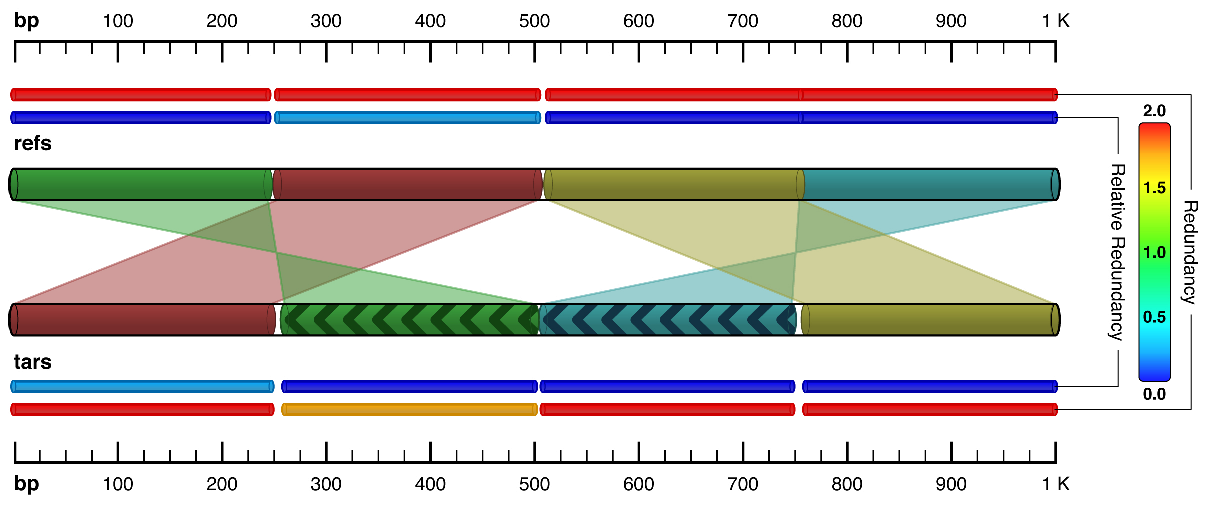
\includegraphics[width=\linewidth]{example.pdf}
  \caption{The result of running Smash++ on ...}
  \label{fig.example}
\end{figure}